\documentclass[a4paper]{article}
\usepackage[spanish]{babel}
\usepackage[utf8]{inputenc}
\usepackage{charter}   % tipografia
\usepackage{graphicx}
%\usepackage{makeidx}
\usepackage{paralist} %itemize inline

%\usepackage{float}
%\usepackage{amsmath, amsthm, amssymb}
%\usepackage{amsfonts}
%\usepackage{sectsty}
%\usepackage{charter}
%\usepackage{wrapfig}
%\usepackage{listings}
%\lstset{language=C}

\usepackage[bookmarks = true, colorlinks=true, linkcolor = black, citecolor = black, menucolor = black, urlcolor = blue]{hyperref} 
\usepackage{color} % para snipets de codigo coloreados
\usepackage{fancybox}  % para el sbox de los snipets de codigo

\definecolor{litegrey}{gray}{0.94}

% \newenvironment{sidebar}{%
% 	\begin{Sbox}\begin{minipage}{.85\textwidth}}%
% 	{\end{minipage}\end{Sbox}%
% 		\begin{center}\setlength{\fboxsep}{6pt}%
% 		\shadowbox{\TheSbox}\end{center}}
% \newenvironment{warning}{%
% 	\begin{Sbox}\begin{minipage}{.85\textwidth}\sffamily\lite\small\RaggedRight}%
% 	{\end{minipage}\end{Sbox}%
% 		\begin{center}\setlength{\fboxsep}{6pt}%
% 		\colorbox{litegrey}{\TheSbox}\end{center}}

\newenvironment{codesnippet}{%
	\begin{Sbox}\begin{minipage}{\textwidth}\sffamily\small}%
	{\end{minipage}\end{Sbox}%
		\begin{center}%
		\vspace{-0.4cm}\colorbox{litegrey}{\TheSbox}\end{center}\vspace{0.3cm}}



\usepackage{fancyhdr}
\pagestyle{fancy}

%\renewcommand{\chaptermark}[1]{\markboth{#1}{}}
\renewcommand{\sectionmark}[1]{\markright{\thesection\ - #1}}

\fancyhf{}

\fancyhead[LO]{Sección \rightmark} % \thesection\ 
\fancyfoot[LO]{\small{Aldasoro Agustina, More \'Angel, Zimenspitz Ezequiel}}
\fancyfoot[RO]{\thepage}
\renewcommand{\headrulewidth}{0.5pt}
\renewcommand{\footrulewidth}{0.5pt}
\setlength{\hoffset}{-0.8in}
\setlength{\textwidth}{16cm}
%\setlength{\hoffset}{-1.1cm}
%\setlength{\textwidth}{16cm}
\setlength{\headsep}{0.5cm}
\setlength{\textheight}{25cm}
\setlength{\voffset}{-0.7in}
\setlength{\headwidth}{\textwidth}
\setlength{\headheight}{13.1pt}

\renewcommand{\baselinestretch}{1.1}  % line spacing


% \setcounter{secnumdepth}{2}
\usepackage{underscore}
\usepackage{caratula}
%\usepackage{url}



% ******************************************************** %
%              TEMPLATE DE INFORME ORGA2 v0.1              %
% ******************************************************** %
% ******************************************************** %
%                                                          %
% ALGUNOS PAQUETES REQUERIDOS (EN UBUNTU):                 %
% ========================================
%                                                          %
% texlive-latex-base                                       %
% texlive-latex-recommended                                %
% texlive-fonts-recommended                                %
% texlive-latex-extra?                                     %
% texlive-lang-spanish (en ubuntu 13.10)                   %
% ******************************************************** %



\begin{document}


\thispagestyle{empty}
\materia{Sistemas Operativos}
\submateria{Primer Cuatrimestre 2015}
\titulo{Trabajo Práctico I}
\subtitulo{Scheduling}
\integrante{Aldasoro Agustina}{86/13}{agusaldasoro@gmail.com}
\integrante{More \'Angel}{931/12}{angel_21_fer@hotmail.com}
\integrante{Zimenspitz Ezequiel}{155/13}{ezeqzim@gmail.com}

\maketitle
\newpage

\thispagestyle{empty}
\vfill
\begin{abstract}
En el presente trabajo se describe la problemática de ...
\end{abstract}


\thispagestyle{empty}
\vspace{3cm}
\tableofcontents
\newpage


%\normalsize
\newpage
\section{Parte I}

\subsection{Ejercicio 1: TaskConsola}
\textit{Programar un tipo de tarea TaskConsola, que simular\'a una tarea interactiva. La tarea debe realizar n llamadas bloqueantes, cada una de una duraci\'on al azar entre bmin y bmax (inclusive). La tarea debe recibir tres par\'ametros: n, bmin y bmax (en ese orden) que ser\'an interpretados como los tres elementos del vector de enteros que recibe la funci\'on.}\\

Al momento de ejecutar la tarea \emph{TaskConsola}, lo que realiza nuestro algoritmo es \emph{uso_IO} n veces (se bloquea n veces), eligiendo cada vez un n\'umero al azar entre \textit{bmin} y \textit{bmax}. Esta elecci\'on se realiza mediante la funci\'on \textit{rand()}, fijando la semilla en srand(time(NULL)) de modo que var\'ia entre ejecuciones seguidas.



\subsection{Ejercicio 2: Ejecuci\'on de tres tareas para TaskConsola}\label{ej2}
\textit{Escribir un lote de 3 tareas distintas: una intensiva en CPU y las otras dos de tipo interactivo (TaskConsola). Ejecutar y graficar la simulaci\'on usando el algoritmo FCFS para 1, 2 y 3 n\'ucleos.}\\

El comportamiento de un Scheduler basado en la t\'ecnica FCFS (First Came, First Served) consiste en ejecutar cada tarea entrante, acorde a su orden de aparici\'on en \textit{ready} sin realizar ninguna interrupci\'on ni cambio de tarea. Cada tarea ejecuta desde su comienzo hasta que finaliza. El lote de tareas que observamos consisti\'o de tres tareas: dos se corresponden el tipo de tarea \textit{TaskConsola} y la restante \textit{TaskCPU} (s\'olo realiza un uso intensivo del CPU -sin bloqueo-). \\

Las tareas utilizadas las siguientes:


	\begin{codesnippet}
	\begin{verbatim}
TaskConsola 4 2 7
TaskCPU 3
@3:
TaskConsola 5 1 10
	\end{verbatim}
	\end{codesnippet}
	
Además, para observar c\'omo varía el tiempo total (si es que lo hace), se simuló la ejecución para 1, 2 y 3 cores. Se le otorg\'o un costo de cambio de contexto de un clock a todos los casos. Dado que en este tipo de Scheduler no hay migración de procesos entre los distintos núcleos, los dem\'as par\'ametros no son de importancia.\\

Los diagramas de Gantt obtenidos fueron los siguientes:\\

 \begin{figure}[h!]
   \begin{center}
 	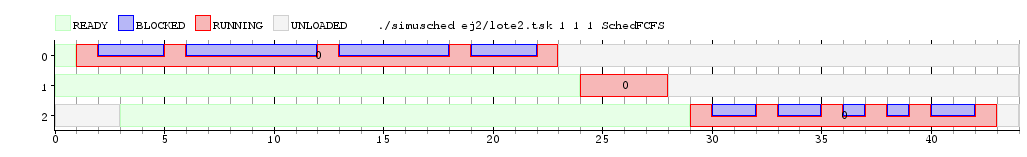
\includegraphics[scale=0.5]{imagenes/ej2/1core.png}
 	\caption{Diagrama de Gantt para la ejecuci\'on del lote de tareas bajo 1 n\'ucleo.}
   \end{center}
 \end{figure} 
 

 \begin{figure}[h!]
   \begin{center}
 	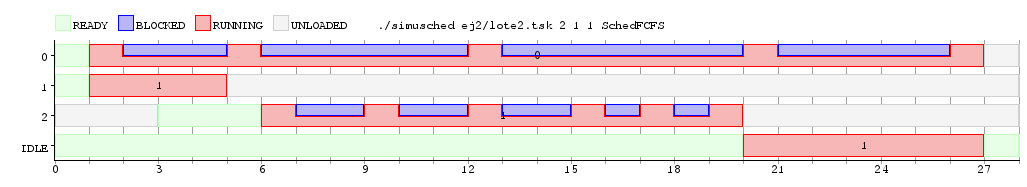
\includegraphics[scale=0.5]{imagenes/ej2/2core.png}
 	\caption{Diagrama de Gantt para la ejecuci\'on del lote de tareas bajo 2 n\'ucleos.}
   \end{center}
 \end{figure} 
 
  \newpage

  \begin{figure}[h!]
   \begin{center}
 	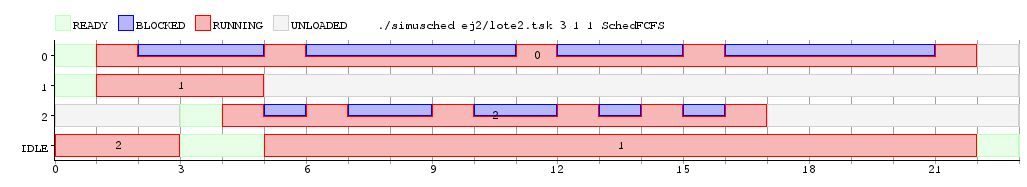
\includegraphics[scale=0.5]{imagenes/ej2/3core.png}
 	\caption{Diagrama de Gantt para la ejecuci\'on del lote de tareas bajo 3 n\'ucleos.}
   \end{center}
 \end{figure} 

 
 Dado a que el algoritmo de Scheduler utilizado es First Come First Served (FCFS), las tareas entrantes se ejecutan secuencialmente por orden de llegada. La ejecuci\'on de ninguna tarea es interrumpida, ya que la tarea ejecuta hasta terminar con su ejecuci\'on, sin tener en cuenta si est\'a bloqueada o no.\\

Conociendo el comportamiento explicado, es coherente que el primer caso (donde se cuenta con un s\'olo n\'ucleo) es donde ejecutar el lote de tres tareas conlleva mayor tiempo. Esto se debe a que el tiempo que demora en ejecutar las tres tareas es la suma de los tiempos de cambio de contexto, el tiempo de ejecuci\'on para cada una y el tiempo que permanece bloqueado.

En cambio, al ejecutarlo con dos o tres n\'ucleos se puede apreciar en los diagramas c\'omo se ejecutan tareas en simult\'aneo. Este comportamiento reduce notablemente el tiempo de ejecuci\'on total, ya que en este caso no ser\'ia la suma del tiempo parcial para cada tarea.\\

A partir de los resultados obtenidos en los gráficos anteriores. Podemos observar que el tiempo total varía de acuerdo al número de cores con los que se este simulando. A medida que se incrementa, el número del tiempo total disminuye. No s\'olo influyó este factor; sino que también, el hecho de que estamos trabajando con un modelo sin desalojo.  
Al trabajar con un solo core debemos esperar que una tarea finalice para que la próxima pueda ser ejecutada. Es decir, se van a ir ejecutando secuencialmente según fueron estando $ready$. \\

Al aumentar en una unidad el número de cores: la primer tarea disponible comenzó a ejecutarse. Dado que aun disponemos de otro core; cuando una segunda tarea pas\'o a estar disponible, pudo ser ejecutada al instante por el núcleo adicional. Y cuando uno de los n\'ucleos se desocupó, se ejecutó la última tarea. Gracias a que dos tareas pudieron ejecutarse simult\'aneamente el tiempo total disminuyó. 

Aún más cuando se trabajó con 3 cores, cada tarea pudo ser ejecutada en un núcleo distinto y como pudieron ejecutarse todas a la vez, el tiempo total fue igual al máximo entre $release$ $time_j$ + $c_j$, donde j indica alguna de las tres tareas utilizadas y $c_j$ su tiempo de ejecución.   

\newpage

\section{Parte II}


\subsection{Ejercicio 3: Scheduler Round-Robin}\label{RoundR}

\textit{Completar la implementaci\'on del scheduler Round-Robin implementando los m\'etodos de la clase SchedRR en los archivos sched_rr.cpp y sched_rr.h. La implementaci\'on recibe, como primer par\'ametro, la cantidad de n\'ucleos y a continuaci\'on los valores de sus respectivos quantums. Debe utilizar una \'unica cola global, permitiendo as\'i la migraci\'on de procesos entre n\'ucleos.}\\


Las estructuras de datos con las que vamos a trabajar, en la clase \emph{SchedRR}, son las siguientes:
	\begin{codesnippet}
	\begin{verbatim}
		int cores;
		vector<int> quantums;
		vector<int> quantums_timer;
		vector<int> actuales;
		int siguiente;
		queue< int, deque<int> > cola;
	\end{verbatim}
	\end{codesnippet}
	
	\begin{itemize}
	\item[•]\textbf{cores} es la cantidad de n\'ucleos.
	\item[•]\textbf{quantums} es un vector de \textit{cores} posiciones, que guarda en quantums[i] el valor del quantum asignado al n\'ucleo i.
	\item[•]\textbf{quantus_timer} es un vector, tal que quantus_timer[i] representa el valor del quantum restante para la tarea corriendo en el n\'ucleo i.
	\item[•]\textbf{actuales} vector que indica el PID de la tarea ejecutandose en el núcleo i (actuales[i]). Para los núcleos sin tarea devuelve la constante $IDLE\_TASK$.
	\item[•]\textbf{siguiente} indica el core al que se le debe asignar la siguiente tarea.
	\item[•]\textbf{cola} es la cola de tareas que restan ser ejecutadas.
	\end{itemize}	
	
%\bigskip	
\noindent  Modificamos a la funcion \emph{next} para que reciba un par\'ametro m\'as (enum Motivo \{ TICK, BLOCK, EXIT \}).
	\begin{codesnippet}
	\begin{verbatim}
    int next(int cpu, const enum Motivo m);
	\end{verbatim}
	\end{codesnippet}
		
\subsubsection*{Constructor Scheduler Round-Robin}		

Al construir un Scheduler Round-Robin, se instancian las estructuras de datos de modo que: se le asigna la cantidad de cores correspondientes (con sus respectivos quantums), todas las tareas actuales se definen como Iddle, la cola est\'a vac\'ia y el siguiente n\'ucleo que le corresponde ejecutar es el primero ingresado como par\'ametro.

\subsubsection*{Funci\'on Load}

Recibe el \emph{pid} de una nueva tarea como par\'ametro. Luego, las primeras n tareas (siendo n el número de cores) se distribuyen entre cada core (dado que al inicio tengo n cores disponibles). Una vez alcanda las n distribuciones se encolan los nuevos \emph{pid} en \emph{cola}. Estos seran asignados a los distintos cores con la función $next$ explicada luego.

\subsubsection*{Funci\'on Tick}	

Recibe \emph{cpu} como par\'ametro y el \emph{Motivo}. Dado que se produjo un tick voy a actualizar el quantum (restarle 1) de la tarea en \emph{cpu}, si no es la Iddle (porque esta corre indefinidamente hasta que la desplace otra tarea). 
Si se acab\'o el quantum de la tarea actual (ya sea porque termin\'o o no) o se bloque\'o, voy a querer actualizar la tarea actual. Para esto, invocó a la funci\'on \emph{next()}. La misma devuelve el \emph{pid} de la próxima tarea a ejecutar en \emph{cpu}.

\subsubsection*{Funci\'on Next}	
	
La funci\'on Next tambi\'en va a ser invocada para un s\'olo n\'ucleo \emph{cpu} pasado por par\'ametro.\\
De este modo, si la tarea que se estaba ejecutando previo a la invocaci\'on de \emph{next()} termin\'o de ejecutarse y la cola se encuentra vac\'ia, la tarea que pondr\'a a ejecutar va a ser la Tarea Iddle.
Si la tarea que se estaba ejecutando no termin\'o su ejecuci\'on o se bloqueo, se deber\'a encolar en la cola global de pendientes.
Si todav\'ia no asign\'e una tarea actual para el n\'ucleo cpu, le asigno la primera de la cola d\'andole todo el quantum disponible para el n\'ucleo \emph{cpu}. (Si la cola se encontraba vac\'ia al llamar la funci\'on next() y la tarea ejecut\'andose no hab\'ia conclu\'ido se la encolar\'a para luego volver a asign\'arsela al n\'ucleo).\\
 
\bigskip 
 
 
 \subsection{Ejercicio 4: Ejecuci\'on de lotes de tareas para Round-Robin}
 
\textit{Dise\~nar uno o m\'as lotes de tareas para ejecutar con el algoritmo del ejercicio anterior. Graficar las simulaciones y comentarlas, justificando brevemente por qu\'e el comportamiento observado es efectivamente el esperable de un algoritmo Round-Robin.}\\


Con el fin de observar el comportamiento del Scheduler basado en la metodolog\'ia Round Robin evaluamos tres casos:

\subsubsection*{Caso 1}

Ejecutamos el mismo lote de tareas utilizado anteriormente (Secci\'on \ref{ej2}), manteniendo los mismos par\'ametros, para as\'i poder evaluar y comparar un Scheduler basado en Round Robin y otro en FCFS. 

	\begin{codesnippet}
	\begin{verbatim}
TaskConsola 4 2 7
TaskCPU 3
@3:
TaskConsola 5 1 10
	\end{verbatim}
	\end{codesnippet}

Los diagramas de Gantt obtenidos fueron los siguientes:\\


 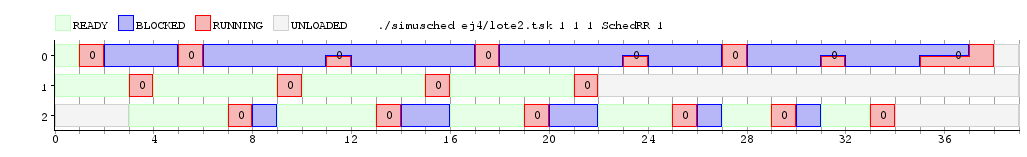
\includegraphics[width=\textwidth,height=3.0in,keepaspectratio]{imagenes/ej4/1core.png} \newline
\begin {flushleft}
\textbf{Figura 4:} Diagrama de Gantt para la ejecuci\'on del lote de tareas bajo 1 n\'ucleo con Scheduler Round Robin.
\end{flushleft}

  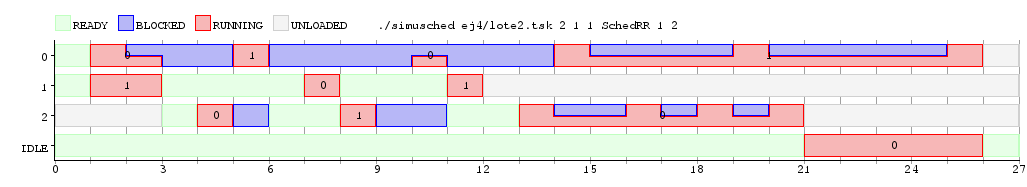
\includegraphics[width=\textwidth,height=3.0in,keepaspectratio]{imagenes/ej4/2core.png} \newline
\begin {flushleft}
\textbf{Figura 5:} Diagrama de Gantt para la ejecuci\'on del lote de tareas bajo 2 n\'ucleos con Scheduler Round Robin.
\end{flushleft}


  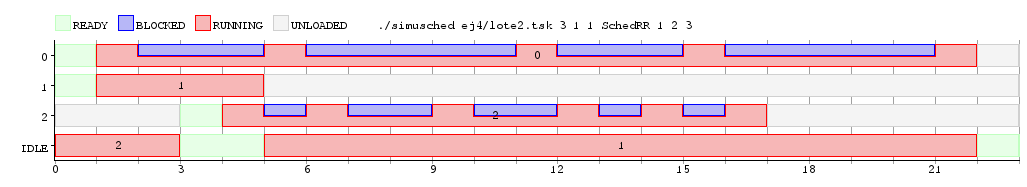
\includegraphics[width=\textwidth,height=3.0in,keepaspectratio]{imagenes/ej4/3core.png} \newline
\begin {flushleft}
\textbf{Figura 6:} Diagrama de Gantt para la ejecuci\'on del lote de tareas bajo 3 n\'ucleos con Scheduler Round Robin.
\end{flushleft}
 
\bigskip 
 
A partir de los resultados obtenidos; podemos ver que, para las \textbf{figuras 5} y \textbf{6}, el tiempo total de ejecución fue el mismo que para las figuras 2 y 3 respectivamente. 

En estos casos, observamos que el tiempo dependió de la tarea \emph{TaskConsola 4 2 7}. La cual ten\'ia el mayor tiempo de ejecución. 

Entonces, sin importar el modelo, aunque las otras dos tareas terminaron, el procesador tuvo que esperar a que finalice dicha tarea.\\

Un caso interesante para análizar es el de las \textbf{figuras 1} y \textbf{4}. En ambas, solo se utilizaba un núcleo pero, en el modelo Round Robin, el tiempo de ejecución fue menor. Esto se debe a que el comportamiento de dicho Scheduler permite cambios de contexto y migración de procesos.

 Para el \emph{modelo FCFS}, había que esperar que una tarea finalice para ejecutar la próxima; si la primera tenía mucho tiempo de bloqueo entonces, ese tiempo se desperciaba. 
 
 En el \emph{modelo Round Robin} se pudieron aprovechar los tiempos que las tareas ocupaban bloqueados para ejecutar otras. Y dado que la tarea con mayor tiempo de ejecución era del tipo TaskConsola, con muchos períodos de bloqueo, el tiempo ``perdido'' fue suficiente para ejecutar las otras tareas en su totalidad.  
 \bigskip
 
 \newpage
 \subsubsection*{Caso 2}\label{caso2}
 
 Para este caso se cre\'o un nuevo lote de tareas y lo que se busco fue: analizar c\'omo varía el tiempo total de ejecución para las mismas, a medida que se cambia el quantum para un total de dos cores.\\
 
 Las tareas que se usaron son las detalladas a continuaci\'on:\\
 \begin{codesnippet}
	\begin{verbatim}
TaskConsola 10 2 6
TaskCPU 10
@3:
TaskCPU 7
@2:
TaskConsola 7 4 10
	\end{verbatim}
	\end{codesnippet}


Los resultados obtenidos fueron:\\

 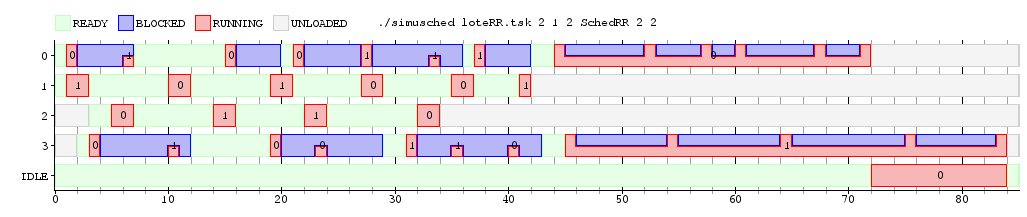
\includegraphics[width=\textwidth,height=3.0in,keepaspectratio]{imagenes/ej4/eje1.png} \\
\begin {flushleft}
\textbf{Figura 7:} Diagrama para la ejecuci\'on del lote de tareas bajo 2 n\'ucleos con quantum de 2 y 2 ciclos respectivamente.
\end{flushleft}

 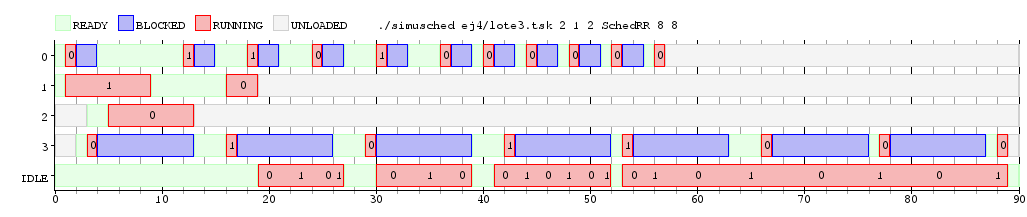
\includegraphics[width=\textwidth,height=3.0in,keepaspectratio]{imagenes/ej4/eje2.png} \\
\begin {flushleft}
\textbf{Figura 8:} Diagrama para la ejecuci\'on del lote de tareas bajo 2 n\'ucleos con quantum de 8 y 8 ciclos respectivamente.
\end{flushleft}


 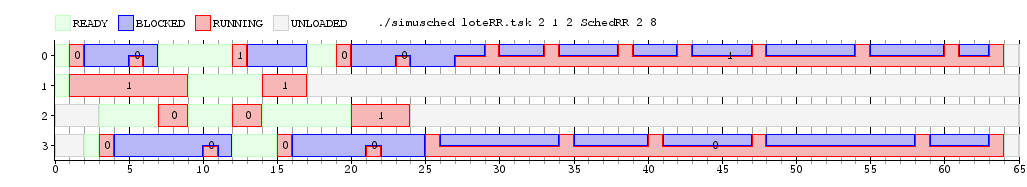
\includegraphics[width=\textwidth,height=3.0in,keepaspectratio]{imagenes/ej4/eje3.png} \\
\begin {flushleft}
\textbf{Figura 9:} Diagrama para la ejecuci\'on del lote de tareas bajo 2 n\'ucleos con quantum de 2 y 8 ciclos respectivamente.
\end{flushleft}

\newpage


Los resultados obtenidos se acercan a lo esperado \textcolor{red}{Poner qu\'e era lo esperado.}: para quantums muy chicos, el tiempo de ejecución total aumenta frente a otros casos (se puede observar dicho comportamiento en la\textbf{ figura 7}).

 Principalmente, cuando se utilizan quantums muy chicos ocurren muchos cambios de contextos. Si su tiempo no es depreciable, aumenta el tiempo total que el procesador necesita para ejecutar todas las tareas. 
 
 Luego, al aumentar el quantum de cada core a 8 (\textbf{figura 8}), observamos que el tiempo total fue menor que para el caso anterior ya que se produjeron menos cambios de contexto. \\
 
 Sin embargo, cuando se usó un quantum bajo y otro de mayor ciclo, el tiempo total bajó con respecto al anterior caso. Podemos atribuir este comportamiento al tipo de tareas con el que trabajamos. 
 
 Como se observa, algunas tareas pudieron migrar en este último caso y finalizar su ejecución más rapidamente. Intuyendo, con estos resultados, que quantums de ciclos muy bajos no son beneficiosos.\\
 
 
  Lo mejor es encontrar un promedio de la cantidad de ciclos para un quantum dado que para valores mas grandes también se observó que puede tardar más con respecto a otros casos.   \\
 
 \bigskip
 
 \subsubsection*{Caso 3}
 
 En el último caso se observó el comportamiento para un lote  de tareas, a medida que modificabamos el número de núcleos en los que se ejecutaban las mismas.\\
 
 Las tareas usadas fueron:
 \begin{codesnippet}
	\begin{verbatim}
TaskCPU 7
@2:
TaskCPU 6
@1:
TaskCPU 10
@3:
TaskCPU 4
	\end{verbatim}
	\end{codesnippet}

	
	Obteniendo los siguientes resultados:\\

  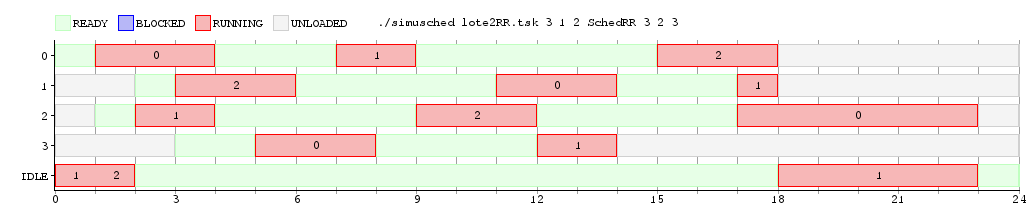
\includegraphics[width=\textwidth,height=3.0in,keepaspectratio]{imagenes/ej4/eje4.png} \\
\begin {flushleft}
\textbf{Figura 10:} Diagrama de Gantt para la ejecuci\'on del lote de tareas bajo 3 n\'ucleos con Scheduler Round Robin.
\end{flushleft}

\newpage

 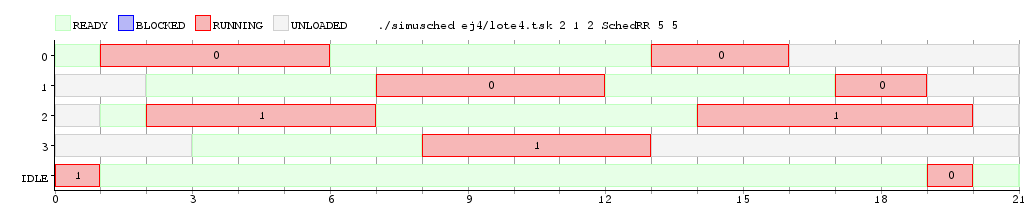
\includegraphics[width=\textwidth,height=3.0in,keepaspectratio]{imagenes/ej4/eje6.png} \\
\begin {flushleft}
\textbf{Figura 11:} Diagrama de Gantt para la ejecuci\'on del lote de tareas bajo 2 n\'ucleos con Scheduler Round Robin.
\end{flushleft}
 
\bigskip 

En este último caso, quisimos comparar el comportamiento de un mismo lote de tareas cuando modificabamos el número de cores bajo un Scheduler Round Robin.\\

 Lo que observamos fue que cuando se contaba con un número mayor de cores, las migraciones de procesos fueron m\'as frecuentes. Debido a que estas no son despreciables -de hecho tienen un costo de 2 ciclos-; al producirse en gran cantidad, el tiempo total para la finalización de tareas aumentó considerablemente. \\
 
 Como se observa en la \textbf{figura 10}, hay un gran lapso de tiempo entre la ejecución de una misma tarea, teniendo en cuenta que en cada quantum se ejecutaron en un core distinto. 
 
 En cambio, en la \textbf{figura 11} no se prudujeron migraciones, y pese a que se contaba con un core menos, el tiempo fue menor. Pudiendo concluir que aunque las migraciones de procesos pueden ser provechosas como se observó en el \emph{Caso 2} (Secci\'on \ref{caso2}), si se producen en exceso pueden perjudicar la perfomance del procesador.  

\newpage

 \subsection{Ejercicio 5: Scheduling algorithms for multiprogramming in a hard-real-time environment}
 
\textit{A partir del art\'iculo Liu, Chung Laung, and James W. Layland. Scheduling algorithms for multiprogramming in a hard-real-time environment. Journal of the ACM (JACM) 20.1 (1973): 46-61.}


\subsubsection{¿Qu\'e problema est\'an intentando resolver los autores?}

Frente al avance que se ven\'ia produciendo esos años en el uso de las computadoras para distintos procesos industriales, los autores establecieron que este comportamiento se iría masificiando aún más y que una correcta aplicación solo es posible cuando se tiene un Scheduler eficiente y factible. Lo consideraron primordial en aquellos usos para los cuales se requerían que las tareas llevadas a cabo se ejecuten dentro de un lapso de tiempo determinado (esto lo llaman \textit{"hard-real-time"}). En caso contrario, una respuesta tardía podría provocar un efecto no deseado en una aplicación o no sería de interés. \\

Otro motivo por el cual intentaron desarollar este tema fue, como describen a lo largo del paper, que hasta entonces estaban orientados a contextos en los que no exist\'ia una cota de tiempo para llevar a cabo todas las tareas. Y los que pose\'ian hacían uso de varios supuestos, llevando a situaciones irreales ciertos casos. \\

Por estos motivos, plantearon dos modelos de Scheduler para tareas en un entorno de \textit{hard-real-time}. Ambos se basan en fijar prioridades para cada una de las tareas: uno de manera estática y el otro dinámicamente. Además para mejorar el rendimiento del mismo, buscan establecer cotas (cuando es posible) para determinar si es aplicable alguno de los modelos de manera que no se produzca \textit{overflow} (alguna de las tareas finalice su ejecución después del tiempo límite).


\subsubsection{¿Por qu\'e introducen el algoritmo de la secci\'on 7? ¿Qu\'e problema buscan resolver con esto?}
En la sección 7 se introduce un nuevo algoritmo, el cual es para un scheduler basado en asignaciones de prioridades dinámicamente (llamado \textit{The deadline Driven Scheduling}). Lo introducen como una variante al algoritmo de prioridades fijas (presentado previamente), intentando evitar o disminuir algunos de los problemas presentados para dicho modelo. \\

Una de los problemas a resolver es mejorar las asignaciones de las prioridades, de manera de aprovechar el procesador a un 100\%. A diferencia del modelo de prioridades fijas, donde la utilización del procesador podía variar de un 70\% a un 100\%. De esta forma, este nuevo algoritmo establece que el nuevo modelo nunca va a ejecutar la Tarea Iddle, sino que siempre se va a estar ejecutando alguna tarea. \\

 Para conseguir esto, se va a aumentar o disminuir la prioridad de una tarea conforme se acerca a su deadline, es decir las prioridades de una misma tarea van a ser modificadas a lo largo de su ejecución. Además, buscaron determinar si un conjunto de tareas evitar\'ia producir overflow, con este algoritmo.\\
 
  En el caso del scheduler con prioridades fijas, se estableció una condición para tal motivo (\textit{teorema 4} \footnote{Scheduling Algorithms for Multiprogramming in a HardReal-Time Environment.
C. L. LIU Project MAC, Massachusetts Institute of Technology AND JAMES W. LAYLAND Jet Propulsion Laboratory, California Institute of Technology. pág 6}), pero esta es s\'olo necesaria. Para el scheduler presentado en esta sección se desarroll\'o una nueva condición, \textit{teorema 7}, la cual garantiza que si se cumple entonces es aplicable el algoritmo y en caso contrario, no lo es (el mismo sera explicado en el siguiente punto). \\
  
 \newpage
\subsubsection{Explicaci\'on coloquial del teorema 7}

Teorema 7:\footnote{Scheduling Algorithms for Multiprogramming in a HardReal-Time Environment.
C. L. LIU Project MAC, Massachusetts Institute of Technology AND JAMES W. LAYLAND Jet Propulsion Laboratory, California Institute of Technology. pág 10}

\textit {For a given set of m tasks, the deadline driven scheduling algorithm
is feasible if and only if }\\
 
 \textit {$(C_1/T_1)$ + $(C_2/T_2)$ + . . . + $(C_m/T_m)$ $\leq$ 1 } \\

\textit{Siendo $C_i$ el tiempo de ejecuci\'on para una tarea i, 1 $\leq$ i $\leq$ m, y $T_i$ su respectivo per\'iodo.}\\

En las secciones anteriores al presente teorema, se determina que la fracción de CPU que utiliza una tarea en el sistema esta dado por $C_i/T_i$ (\textit{the utilization factor}). Lo que se plantea en este teorema es que un Scheduler, para una cantidad m de tareas, es factible y por lo tanto realizable sin que se produzca overflow cuando la suma del costo de CPU de cada tarea es menor que uno o igual a 1. Es decir que el ejecutar todas las tareas este dentro de la capacidades del CPU (no supere el 100\% del rendimiento del mismo), ya que en caso contrario se estaria exigiendo que el CPU trabaje a un l\'imite mayor, lo cual es imposible. \\




\subsubsection{Scheduler}
\textit{Dise\~nar e implementar un scheduler basado en prioridades fijas y otro en prioridades din\'amicas. Para eso, complete las clases SchedFixed y SchedDynamic que se encuentran en los archivos sched fixed.[h|cpp] y sched dynamic.[h|cpp] respectivamente.}\\

\subsection*{Implementaciones:}

\subsection*{Scheduler con prioridades fijas:}

Las estructuras de datos con las que vamos a trabajar, en la clase \emph{SchedFixed}, son las siguientes:
	\begin{codesnippet}
	\begin{verbatim}
struct datos{
    int pid;
    int periodo;
    bool operator< (const datos& otro) const{
        return otro.periodo <= periodo;
    }
};
		
vector<int> periodos;
priority_queue<datos> pq;
	\end{verbatim}
	\end{codesnippet}
	
	\begin{itemize}
	\item[•]\textbf{struct datos} Diseñado para representar a una tarea, en él se podra encontrar el PID y el período de la misma.
	\item[•]\textbf{periodos} vector donde cada posición representa un PID (dado que estos se enumeran desde el cero y se van incrementando en uno) en las mismas se encuentra el período que le fue asignado a cada tarea.
	\item[•]\textbf{pq} cola de prioridad de datos donde la prioridad más alta la tiene aquel dato cuyo periodo es el menor. Dado que se esta implementando el scheduler con prioridades fijas, en él se atribuye que la prioridad esta dada por:\newline
	$prioridad$ = $1 / periodo$ \newline 
	Es decir a menor periodo mayor prioridad, es por esto que la cola siempre va a devolver como primer elemento el más priorítario respecto del per\'iodo m\'inimo.
	\end{itemize}	
	
		
\subsubsection*{Inicializando Scheduler Fixed, función initizalize}		

Al construir el Scheduler basado en prioridades fijas, como primer medida se inizializó \emph{periodos}, el mismo contiene el per\'iodo asignado a cada tarea. Para esto, se utilizó la función \emph{period} de esta manera en cada posición guardamos el correspondiente per\'iodo asignado.

\subsubsection*{Funci\'on Load}

Recibe el \emph{pid} de una nueva tarea como par\'ametro. Procede a crear una tarea del tipo \emph{datos} con el \emph{pid} recibido y el per\'iodo del mismo que se puede obtener de \emph{periodos} (\emph{periodos[pid]}). Finalizado esto, se encola la tarea en \emph{pq}.

\subsubsection*{Funci\'on Tick}	

Recibe \emph{cpu} como par\'ametro y el \emph{Motivo}. Dado que se produjo un tick, se procede a actualizar (de ser necesario) la asignación del \emph{cpu} para las distintas tareas.  Es por esto, que si la tarea que se estaba ejecutando hasta entonces terminó, o si se estaba ejecutando la IDDLE, y existe otra tarea en \emph{pq}; la próxima a ejecutar será la primera de ella (la de menor período), en caso contrario se ejecutara la IDDLE. 

En el caso de no haber terminado la tarea, se procede a encolarla en \emph{pq}. Si existe una tarea con mayor priodidad, ser\'a devuelta como próxima a ejecutar y sino ser\'a la misma que se acab\'o de encolar. \\ 


 
\bigskip 

\subsection*{Scheduler con prioridades dinámicas:}

Las estructuras utilizadas, en la clase \emph{SchedDynamic}, son las siguientes:
	\begin{codesnippet}
	\begin{verbatim}
struct datos{
    int pid;
    int deadline;
    bool operator< (const datos& otro) const{
        return otro.deadline <= deadline; 
    }
};

priority_queue<datos> pq;
datos actual;
bool primera;
	\end{verbatim}
	\end{codesnippet}
	
	\begin{itemize}
	
	\item[•]\textbf{struct datos} Al igual que para el scheduler anterior, est\'a diseñado para representar a una tarea. En él, se encontrar\'a el \emph{PID} y el \emph{per\'iodo} de la misma.
	\item[•]\textbf{pq} cola de prioridad de \emph{datos} donde la prioridad más alta la tiene aquel cuyo deadline sea el menor. Como se est\'a implementando un scheduler con prioridades dinámicas, en el mismo se atribuye que la prioridad mas álta la tiene aquella tarea cuyo deadline esta mas próximo a finalizar. Por lo que \emph{pq} va a devolver como primer elemento (el de mayor prioridad) a la tarea con deadline m\'inimo.
	\item[•]\textbf{actual} va a representar a la tarea ejecutandose actualmente.
	\item[•]\textbf{primera} Se utiliza para saber si hay una tarea asignada a \emph{actual}, la misma se inicializa con True en el constructor.
	\end{itemize}	
	
\subsubsection*{Inicializando Scheduler Dynamic, función initizalize}		
		
\textcolor{red}{Falta funcion de Inicializar}\\

\subsubsection*{Funci\'on Load}

Recibe el \emph{pid} de una nueva tarea como par\'ametro y procede a crear la tarea asociada a ese \emph{pid}, el deadline de la misma ser\'a (inicialmente) su per\'iodo. Finalizado esto, se encola la tarea en \emph{pq}. En caso de que \emph{primera} sea true, se le asigna a \emph{actual} esta última tarea creada.

\subsubsection*{Funci\'on Tick}	

Recibe \emph{cpu} como par\'ametro y el \emph{Motivo}. Al producirse un tick se procede a actualizar la asignación del \emph{cpu} para las distintas tareas.  Si la que se estaba ejecutando hasta entonces terminó, o si se estaba ejecutando la IDDLE, y existe otra tarea en \emph{pq}: la primer tarea de la cola será la próxima a ejecutar (la de menor deadline), en caso contrario se ejecutara la IDDLE. En el caso de no haber terminado la tarea, se procede a encolar a \emph{actual} en \emph{pq} pero, disminuyendo su deadline en uno ya que la tarea completo un TICK. Si existe una tarea con mayor prioridad, ser\'a devuelta como próxima a ejecutar y sino, ser\'a la misma que se acaba de encolar.  




\newpage
\section{Parte III}


 \subsection{Ejercicio 6: TaskBatch}
\textit{Programar un tipo de tarea TaskBatch que reciba dos par\'ametros: total_cpu y cant_bloqueos. Una tarea de este tipo deber\'a realizar cant bloqueos llamadas bloqueantes, en momentos elegidos pseudoaleatoriamente. En cada tal ocasi\'on, la tarea deber\'a permanecer bloqueada durante exactamente un (1) ciclo de reloj. El tiempo de CPU total que utilice una tarea TaskBatch deber\'a ser de total cpu ciclos de reloj (incluyendo el tiempo utilizado para lanzar las llamadas bloqueantes; no as\'i el tiempo en que la tarea permanezca bloqueada).}\\

Nuestra funci\'on arma un vector de \emph{cant_bloqueos} posiciones y les asigna para cada una: un valor pseudoaleatorio, sin repetidos, dentro de su rango de tiempo de ejecuci\'on \emph{total_cpu}. A estos valores se los ordena dentro del arreglo para poder recorrerlo secuencialmente.\\

Luego, para cada ciclo de clock se pregunta si ese momento est\'a indicado para realizar una llamada bloqueante. En caso afirmativo, se ejecuta \textit{uso_IO(pid, 1)}; en caso contrario, \textit{uso_CPU(pid, 1)}.\\

Debemos aclarar que nuestro algoritmo est\'a definido s\'olo para casos donde alcanzan los clocks para ejecutar las llamadas bloqueantes requeridas (el caso contrario no nos es de inter\'es).

\bigskip 
 \subsection{Ejercicio 7: Ejecuci\'on lote de tareas TaskBatch}
\textit{Elegir al menos dos m\'etricas diferentes, definirlas y explicar la sem\'antica de su definici\'on. Dise\~nar un lote de tareas TaskBatch, todas ellas con igual uso de CPU, pero con diversas cantidades de bloqueos. Simular este lote utilizando el algoritmo SchedRR y una variedad apropiada de valores de quantum. Mantener fijo en un (1) ciclo de reloj el costo de cambio de contexto y dos (2) ciclos el de migraci\'on. Deben variar la cantidad de n\'ucleos de procesamiento. Para cada una de las m\'etricas elegidas, concluir cu\'al es el valor \'optimo de quantum a los efectos de dicha m\'etrica.}\\



Las m\'etricas elegidas fueron: Tiempo de Respuesta y TournAround.\\

%Las m\'etricas elegidas fueron: Tiempo de Respuesta, TournAround y Waiting Time.\\

\underline{\emph{Tiempo de Respuesta}}: Tiene en cuenta el tiempo que tarda cada proceso en empezar a ejecutarse desde su primera aparici\'on en \textit{ready}. Cuanto menor tiempo de Respuesta tienen los procesos, el usuario adquiere una mayor interactividad.\\

\underline{\emph{TournAround}}: Tiene en cuenta el tiempo que utiliza un proceso en ejecutarse completamente, es decir desde su primera aparici\'on en \textit{ready} hasta que termina su ejecuci\'on.\\

%\underline{\emph{Waiting Time}}: Tiene en cuenta todo el tiempo que el proceso se encuentra en estado Ready (desde que es lanzado hasta su finalizaci\'on).\\


El lote de Tareas TaskBatch dise\~nado es el siguiente:
	\begin{codesnippet}
	\begin{verbatim}
TaskBatch 25 3
TaskBatch 25 7
@3:
TaskBatch 25 0
@5:
TaskBatch 25 10
@7:
TaskBatch 25 5
@10:
TaskBatch 25 9
	\end{verbatim}
	\end{codesnippet}

	Ejecutamos este lote de tareas, considerando diferentes cantidades de n\'ucleos variando dentro de ellas el quantum de cada uno (En los casos A se eligieron los quantums m\'as chicos, en los C los m\'as grandes y en los B los intermedios). En cada caso, tomamos el promedio de los valores de \textit{Tiempo de Respuesta} y \textit{TournAround} para luego comparar cualitativamente.
	
	Para cada caso a tratar, ejecutamos 100 veces el mismo comando para luego sacar un promedio de las mediciones hechas ya que estamos trabajando con n\'umeros (pseudo)random. Exponemos un ejemplo tomado de cada caso a continuaci\'on:
	
	\subsubsection*{1 N\'ucleo}
	
	\textbf{Caso A:} El quantum de este n\'ucleo es de 3 clocks.
	
	 \begin{figure}[h!]
   \begin{center}
 	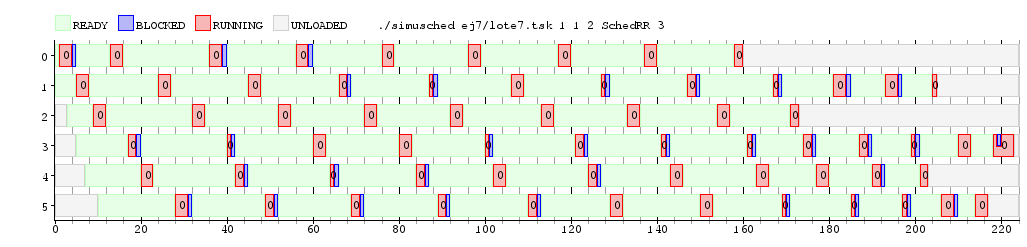
\includegraphics[scale=0.5]{imagenes/ej7/1nucleoA.png}
 	\textbf{Tiempo de Respuesta:} 9.166666667\\
 	\textbf{Tiempo de TournAround:} 192.6666667\\
 %	\textbf{Waiting Time Promedio:} \\
   \end{center}
 \end{figure} 
	
	
	\textbf{Caso B:} El quantum de este n\'ucleo es de 10 clocks.
	
		 \begin{figure}[h!]
   \begin{center}
 	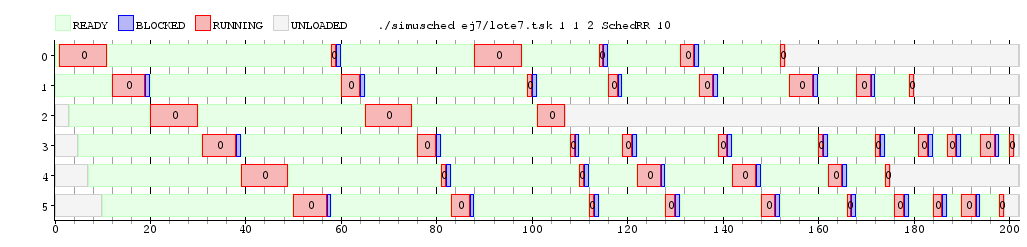
\includegraphics[scale=0.5]{imagenes/ej7/1nucleoB.png}
 	\textbf{Tiempo de Respuesta:} 18.5 \\
 	\textbf{Tiempo de TournAround:} 152.8333333\\
 %	\textbf{Waiting Time Promedio:} \\
   \end{center}
 \end{figure} 
	
	\textbf{Caso C:} El quantum de este n\'ucleo es de 25 clocks.

		 \begin{figure}[h!]
   \begin{center}
 	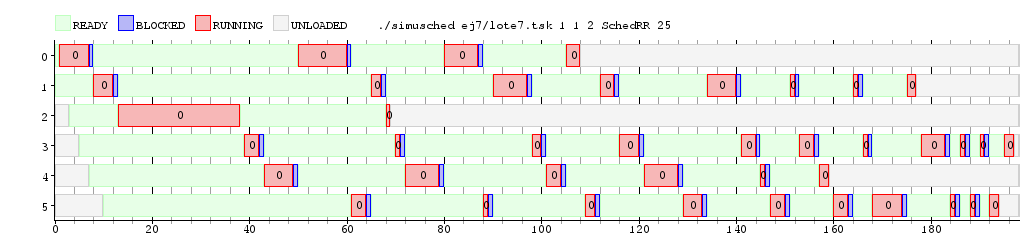
\includegraphics[scale=0.5]{imagenes/ej7/1nucleoC.png}
 	\textbf{Tiempo de Respuesta:} 26.66666667 \\
 	\textbf{Tiempo de TournAround:} 142.5 \\
 %	\textbf{Waiting Time Promedio:} \\
   \end{center}
 \end{figure} 	
	
\newpage	
	\subsubsection*{2 N\'ucleos}
	
	\textbf{Caso A:} Un quantum es de 3 y el otro de 5 clocks.

		 \begin{figure}[h!]
   \begin{center}
 	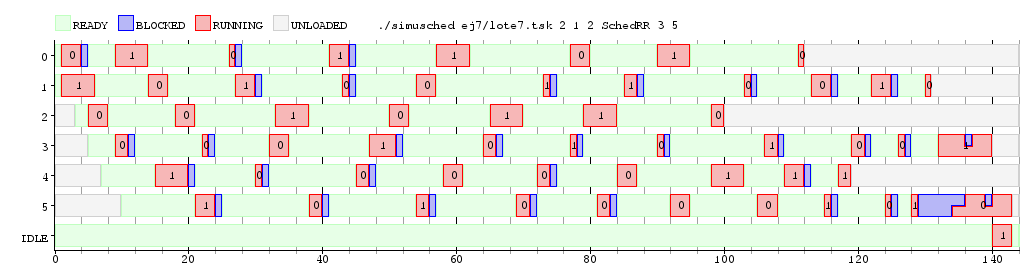
\includegraphics[scale=0.5]{imagenes/ej7/2nucleoA.png}
 	\textbf{Tiempo de Respuesta:} 4.5 \\
 	\textbf{Tiempo de TournAround:} 120 \\
 	%\textbf{Waiting Time Promedio:} \\
   \end{center}
 \end{figure} 
 	
	\textbf{Caso B:} Los dos quantums son de 10 clocks.

		 \begin{figure}[h!]
   \begin{center}
 	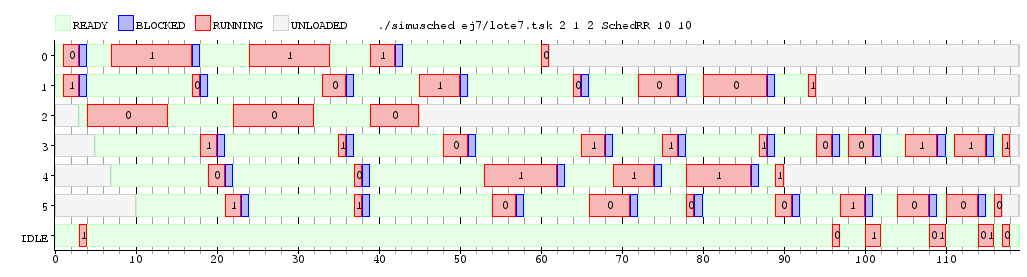
\includegraphics[scale=0.5]{imagenes/ej7/2nucleoB.png}
 	\textbf{Tiempo de Respuesta:} 6.333333333\\
 	\textbf{Tiempo de TournAround:} 94.5\\
 %	\textbf{Waiting Time Promedio:} \\
   \end{center}
 \end{figure} 
 	
	\textbf{Caso C:} Los dos quantums son de 25 clocks.

		 \begin{figure}[h!]
   \begin{center}
 	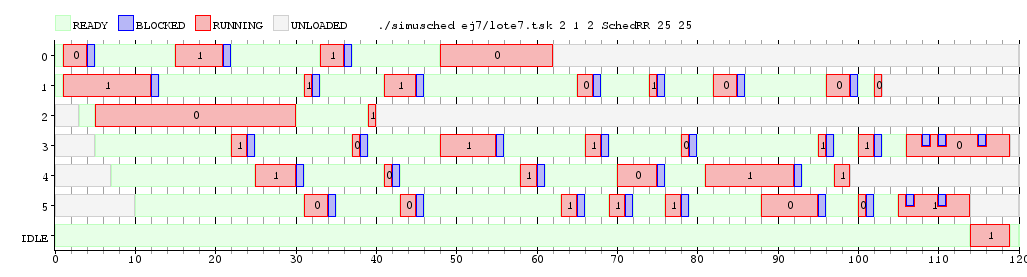
\includegraphics[scale=0.5]{imagenes/ej7/2nucleoC.png}
 	\textbf{Tiempo de Respuesta:} 10 \\
 	\textbf{Tiempo de TournAround:} 85.33333333 \\
 %	\textbf{Waiting Time Promedio:} \\
   \end{center}
 \end{figure} 
 
 \newpage
	\subsubsection*{3 N\'ucleos}
	
	\textbf{Caso A:} Los quantums son de: 3, 5 y 7 clocks.

		 \begin{figure}[h!]
   \begin{center}
 	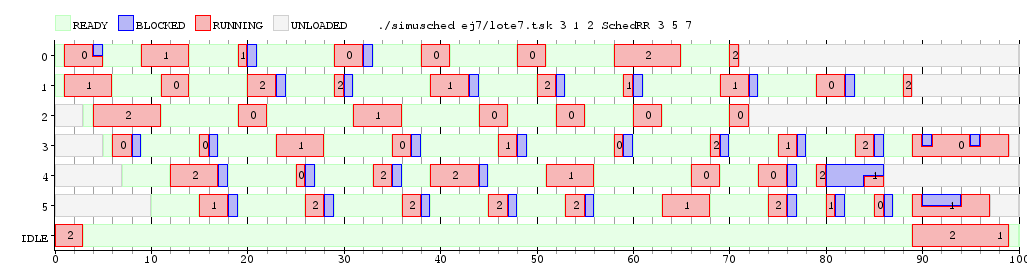
\includegraphics[scale=0.5]{imagenes/ej7/3nucleoA.png}
 	\textbf{Tiempo de Respuesta:} 2.333333333 \\
 	\textbf{Tiempo de TournAround:} 81.5 \\
 %	\textbf{Waiting Time Promedio:} \\
   \end{center}
 \end{figure} 
 	
	\textbf{Caso B:}  Los quantums son de: 10, 10 y 5 clocks.

		 \begin{figure}[h!]
   \begin{center}
 	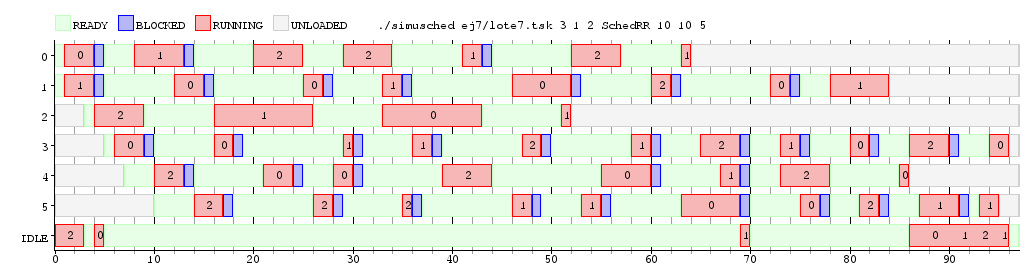
\includegraphics[scale=0.5]{imagenes/ej7/3nucleoB.png}
 	\textbf{Tiempo de Respuesta:} 2.166666667 \\
 	\textbf{Tiempo de TournAround:} 72.66666667 \\
 %	\textbf{Waiting Time Promedio:} \\
   \end{center}
 \end{figure} 
 	
	\textbf{Caso C:}  Los quantums son de: 25, 25 y 10 clocks.

		 \begin{figure}[h!]
   \begin{center}
 	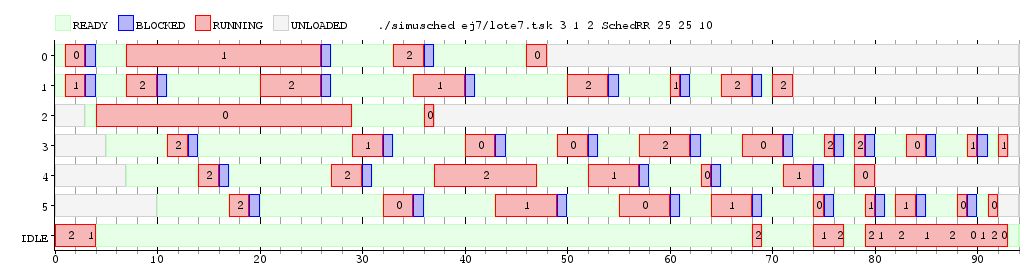
\includegraphics[scale=0.5]{imagenes/ej7/3nucleoC.png}
 	\textbf{Tiempo de Respuesta:} 2.666666667 \\
 	\textbf{Tiempo de TournAround:} 62.33333333 \\
 %	\textbf{Waiting Time Promedio:} \\
   \end{center}
 \end{figure} 
 
 \newpage
	\subsubsection*{4 N\'ucleos}
	
	\textbf{Caso A:}  Los quantums son de: 3, 5, 7 y 10 clocks.
	
		 \begin{figure}[h!]
   \begin{center}
 	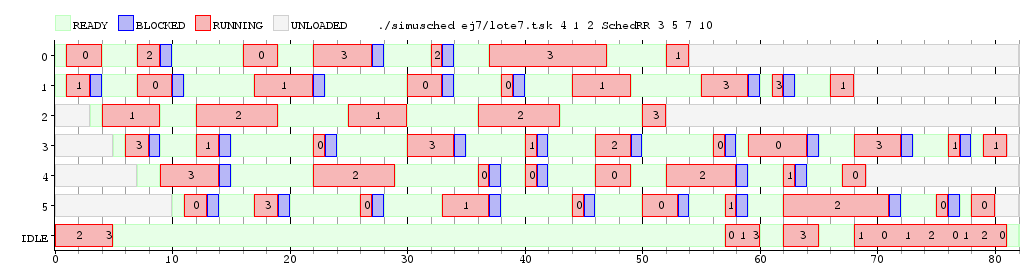
\includegraphics[scale=0.5]{imagenes/ej7/4nucleoA.png}
 	\textbf{Tiempo de Respuesta:} 1.333333333 \\
 	\textbf{Tiempo de TournAround:} 57.16666667 \\
 %	\textbf{Waiting Time Promedio:} \\
   \end{center}
 \end{figure} 
 	
	\textbf{Caso B:}  Los quantums son de: 10, 10, 5 y 5 clocks.
	
			 \begin{figure}[h!]
   \begin{center}
 	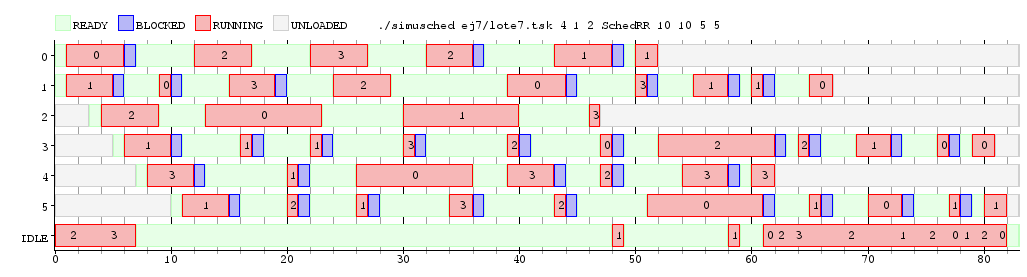
\includegraphics[scale=0.5]{imagenes/ej7/4nucleoB.png}
 	\textbf{Tiempo de Respuesta:} 1.333333333 \\
 	\textbf{Tiempo de TournAround:} 53 \\
 %	\textbf{Waiting Time Promedio:} \\
   \end{center}
 \end{figure} 
 
	\textbf{Caso C:}  Los quantums son de: 25, 25, 10 y 25 clocks.
	
			 \begin{figure}[h!]
   \begin{center}
 	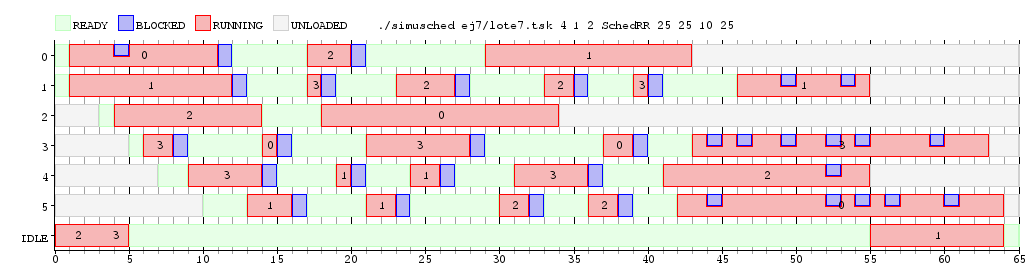
\includegraphics[scale=0.5]{imagenes/ej7/4nucleoC.png}
 	\textbf{Tiempo de Respuesta:} 1.5 \\
 	\textbf{Tiempo de TournAround:} 48.16666667 \\
 %	\textbf{Waiting Time Promedio:} \\
   \end{center}
 \end{figure} 
 
 \newpage
	\subsubsection*{6 N\'ucleos}
	
	\textbf{Caso A:}  Los quantums son todos de 1 clock.

		 \begin{figure}[h!]
   \begin{center}
 	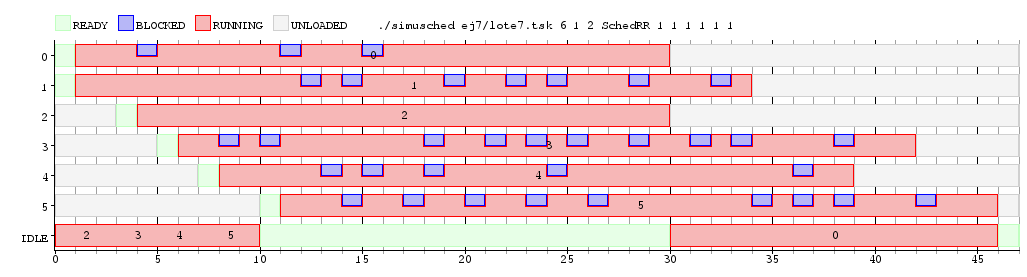
\includegraphics[scale=0.5]{imagenes/ej7/6nucleoA.png}
 	\textbf{Tiempo de Respuesta Promedio:} 1 \\
 	\textbf{Tiempo de TournAround Promedio:} 32.66666667 \\
 %	\textbf{Waiting Time Promedio:} \\
   \end{center}
 \end{figure} 
 	
	\textbf{Caso B:}  Los quantums son de: 10, 10, 5, 5, 10, 5 clocks.
	
			 \begin{figure}[h!]
   \begin{center}
 	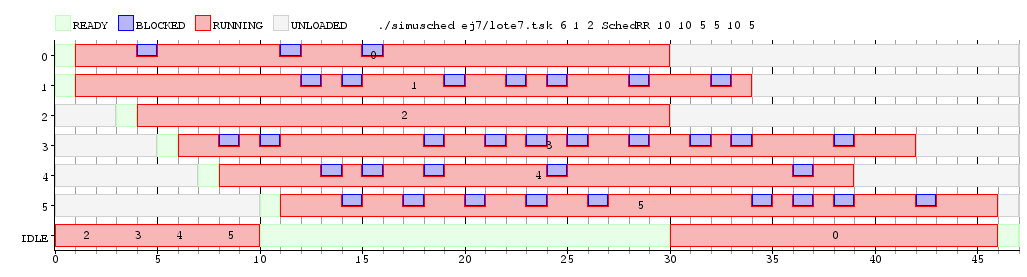
\includegraphics[scale=0.5]{imagenes/ej7/6nucleoB.png}
 	\textbf{Tiempo de Respuesta Promedio:} 1 \\
 	\textbf{Tiempo de TournAround Promedio:} 32.66666667 \\
 %	\textbf{Waiting Time Promedio:} \\
   \end{center}
 \end{figure} 
 
	\textbf{Caso C:}  Los quantums son todos de 25 clocks.
	
		 \begin{figure}[h!]
   \begin{center}
 	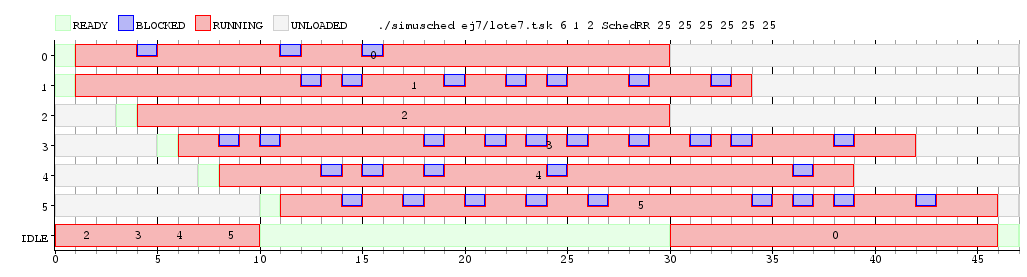
\includegraphics[scale=0.5]{imagenes/ej7/6nucleoC.png}
 	\textbf{Tiempo de Respuesta Promedio:} 1 \\
 	\textbf{Tiempo de TournAround Promedio:} 32.66666667 \\
 %	\textbf{Waiting Time Promedio:} \\
   \end{center}
 \end{figure} 

\newpage

Luego graficamos los tiempos obtenidos, con el fin de tener una herramienta m\'as declarativa para la comparaci\'on de casos bajo las dos m\'etricas usadas.

\subsubsection*{M\'etrica de Tiempo de Respuesta}

Graficamos los promedios de tiempo de respuesta.
		 \begin{figure}[h!]
   \begin{center}
 	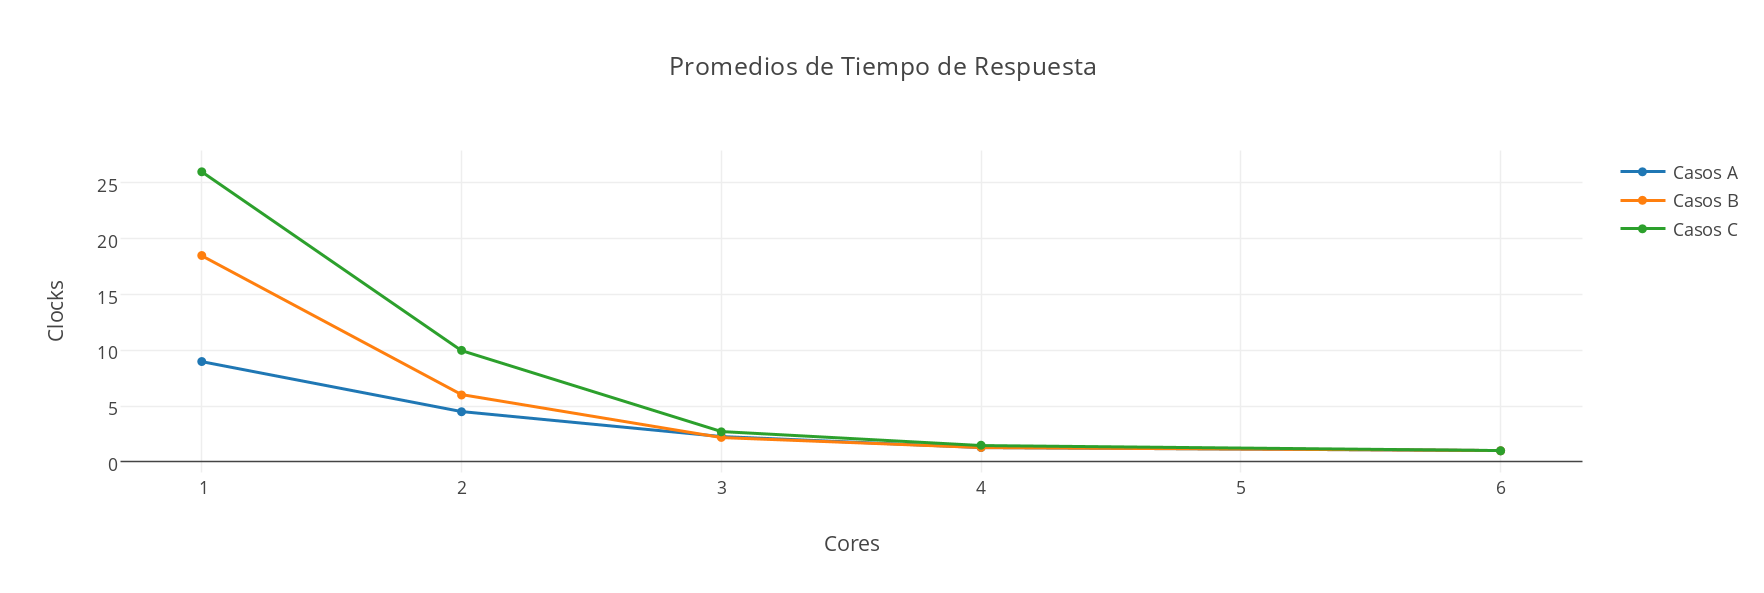
\includegraphics[scale=1.2]{imagenes/ej7/TiemposResp.png}
   \end{center}
 \end{figure} 
 
 Acorde a lo que resulta intuitivo, estos valores siempre descienden acorde aumenta la cantidad de cores. Los casos con una cantidad de n\'ucleos mayor a seis fueron descartados, ya que resultan triviales dado a que la cantidad de tareas es seis (son an\'alogos al caso de 6 n\'ucleos dejando el resto ejecutando la Tarea Iddle).
 
 En el gr\'afico se puede apreciar la relaci\'on que preservan los casos A, B y C indiferentemente de la cantidad de n\'ucleos existentes: los casos con quantum de mayor tama\~no arrojaron valores m\'as altos. Este comportamiento se debe a que, al momento de ingresar una tarea debe esperar a que alg\'un core quede libre (es decir, la tarea que estaba ejecutando haya terminado su quantum o quede bloqueada).
 
 En los casos donde la cantidad de tareas es menor o igual a la cantidad de n\'ucleos, el promedio de los tiempos de respuesta siempre va a ser el tiempo que tarde en cargarse una tarea. En nuestro caso este tiempo es 1 clock.\\
 
 De este modo, podemos definir que para tiempos de respuesta \'optimos no s\'olo debemos contar con la mayor cantidad de n\'ucleos posibles (siempre menor igual o a la cantidad de tareas, ya que una cantidad mayor carece de mejoras) sino que tambi\'en con (al menos un) core que tenga un quantum de tama\~no peque\~no. Esto nos asegura que al momento de ingresar una nueva tarea, el tiempo que debe esperar hasta que alg\'un core quede libre es menor.

\newpage

\subsubsection*{M\'etrica de TournAround}
Graficamos los promedios de tiempos de TournAround.

 		 \begin{figure}[h!]
   \begin{center}
 	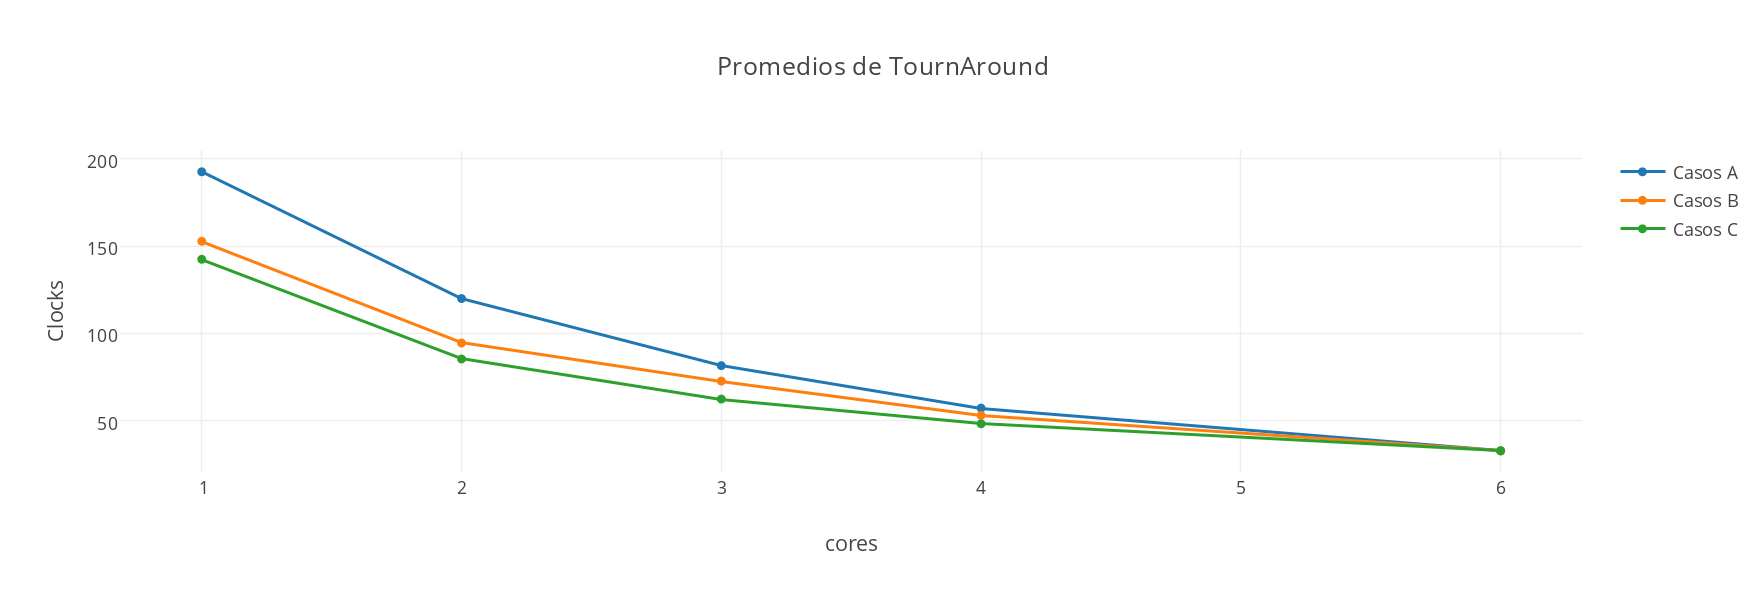
\includegraphics[scale=1.2]{imagenes/ej7/TiemposTournAround.png}
   \end{center}
 \end{figure} 
 
En primera instancia, debemos marcar que el hecho de que la cantidad de cores sea igual a la cantidad de tareas no s\'olo otorga un tiempo peque\~no sino que es el \'optimo ya que al poseer m\'as n\'ucleos estos quedar\'ian libres ejecutando continuamente la Tarea Iddle. Resulta intuitivo marcar que acorde aumenta la cantidad de cores, descienden los promedios de tiempos ya que cada tarea tiene su n\'ucleo para ejecutar sin importar el quantum debido a que nadie la va a desalojar.\\


Bajo esta m\'etrica, la relaci\'on que se preserva entre los casos A, B y C es inversamente proporcional a la m\'etrica anterior. Contando con quantums m\'as peque\~nos, el tiempo que lleva ejecutar una tarea en total es menor ya que se ejecuta con una frecuencia m\'as alta. Hay que tener en cuenta que contar con quantums menor es beneficioso en todos los casos mostrados, ya que se us\'o un tiempo de cambio de contexto de 2 clocks lo que resulta un tiempo peque\~no.\\

\bigskip
 
En el caso de ambas m\'etricas tratadas, se utilizaron la ejecuci\'on de cada caso 100 veces. Esto independiza los gr\'aficos obtenidos de los bloqueos que pudieron ser causados, ya que fueron elegidos aleatoriamente. 
 
 \newpage
 \subsection{Ejercicio 8: Scheduler Round-Robin modificado}
 
\textcolor{red}{(ME FALTA EXPLICAR ESTAS EXPERIMENTACIONES, PERO VOY A ESTUDIAR PARA METODOS :/ )} \\
 
\textit{Implemente un scheduler Round-Robin que no permita la migraci\'on de procesos entre n\'ucleos (SchedRR2). La asignaci\'on de CPU se debe realizar en el momento en que se produce la carga de un proceso (load). El n\'ucleo correspondiente a un nuevo proceso ser\'a aquel con menor cantidad de procesos activos totales (RUNNING + BLOCKED + READY). Dise\~ne y realice un conjunto de experimentos que permita evaluar comparativamente las dos implementaciones de Round-Robin.}\\


Las estructuras de datos con las que vamos a trabajar, en la clase \emph{SchedRR2}, son las siguientes:


	\begin{codesnippet}
	\begin{verbatim}
		int cores;
		vector<int> quantums;
		vector<int> quantums_timer;
		vector<int> actuales;
		int siguiente;
		vector<pair<int, queue<int, deque<int>>*>> colas;
	\end{verbatim}
	\end{codesnippet}
	
	\begin{itemize}
	\item[•]\textbf{cores} cantidad de n\'ucleos.
	\item[•]\textbf{quantums} vector de \emph{cores} posiciones, donde quantums[i] es el valor del quantum asignado al core i.
	\item[•]\textbf{quantus_timer}  vector tal que en quantus_timer[i] se encuentra el valor del quantum restante para la tarea corriendo en el i-esimo núcleo.
	\item[•]\textbf{actuales} vector que indica el PID de la tarea ejecutandose en el núcleo i (actuales[i]). Para los núcleos sin tarea devuelve la constante \textit{IDLE\_TASK}.
	\item[•]\textbf{siguiente} indica el core al que se le debe asignar la próxima tarea.
	\item[•]\textbf{colas} vector de tuplas. Donde cada posición reresenta a un core y la primer componente de la tupla hacer referencia al número de tareas running + blocked + ready en el mismo. Y la segunda componente es una cola FIFO con los respectivos PID's.  
	\end{itemize}	
	
%\bigskip	
\noindent  Modificamos a la funcion \emph{next} para que reciba un parametro m\'as (enum Motivo \{ TICK, BLOCK, EXIT \}).
	\begin{codesnippet}
	\begin{verbatim}
    int next(int cpu, const enum Motivo m);
	\end{verbatim}
	\end{codesnippet}
		
\subsubsection*{Constructor Scheduler Round-Robin Modificado}		

Al construir un Scheduler Round-Robin sin migración de procesos, empezamos por instanciar las estructuras de datos de modo que: a \emph{cores} se le asigna la cantidad de cores correspondientes. A \emph{quantums\_timer} los respectivos quantums; Todas las tareas actuales se definen como Iddle en \emph{actuales}; Se inicia cada tupla de \emph{colas} en cero ya que aún no hay tareas y las colas vacias; Por último \emph{siguiente} es el n\'ucleo al que le corresponde ejecutar la primer tarea, es decir al 0.

\subsubsection*{Funci\'on Load}

Recibe el \emph{pid} de una nueva tarea como par\'ametro. Al igual que para el Scheduler Round Robin, adoptamos distribuir las primeras n tareas entre cada core (dado que al inicio hay n cores disponibles). Además, se incrementa la primer componente de cada tupla en uno (ahora en cada core tengo una tarea).

 Una vez alcanzadas las n distribuciones de las futuras tareas, ser\'an asignadas a los CPU's con menor cantidad de tareas \emph{running + blocked + ready}.  Es decir, se encolar\'an sus pid's en las colas de cada CPU de \emph{colas} con la primer componente más baja, incrementado ahora dicha componente.

\subsubsection*{Funci\'on Tick}	

Recibe \emph{cpu} como par\'ametro y el \emph{Motivo}. Dado que se produjo un tick, voy a actualizar el quantum (restarle 1) de la tarea en \emph{cpu}, siempre que no sea la IDLE. Si se acab\'o el quantum de la tarea actual (ya sea porque termin\'o o no) o se bloque\'o, voy a querer actualizar la tarea actual. Invocando a la funci\'on \emph{next()}. La misma devuelve el \emph{pid} de la próxima tarea a ejecutar en \emph{cpu}.

\subsubsection*{Funci\'on Next}	
	

Si la tarea que se estaba ejecutando previo a la invocaci\'on de \emph{next()} termin\'o de ejecutarse y la cola se encuentra vac\'ia, la tarea que pondr\'a a ejecutar va a ser la Tarea Iddle y se actualiza el número que indica cuantas tareas hay en ese cpu.

Si la tarea que se estaba ejecutando no termin\'o su ejecuci\'on o se bloqueo, se deber\'a encolar en la cola del \emph{cpu} pasado por parametro.

Si todav\'ia no asign\'e una tarea actual para el mismo, le asigno la primera de la cola d\'andole todo el quantum disponible para el n\'ucleo \emph{cpu}. (Si la cola se encontraba vac\'ia al llamar la funci\'on next() y la tarea ejecut\'andose no hab\'ia conclu\'ido se la encolar\'a para luego volver a asign\'arsela al n\'ucleo).\\
 
\bigskip 
 
Para evaluar el comportamiento del Scheduler Round Robin sin migraciones frente al diseñado en la Sección \ref{RoundR}, vamos a utilizar el mismo lote de tareas que se us\'o para este último en los casos 2 y 3. Manteniendo las mismas condiciones en las que fueron obtenidos los resultados.\\


De esta forma para el lote de tareas:
 
 \begin{codesnippet}
	\begin{verbatim}
TaskConsola 10 2 6
TaskCPU 10
@3:
TaskCPU 7
@2:
TaskConsola 7 4 10
	\end{verbatim}
	\end{codesnippet}
	
Se obtuvo como resultado:	

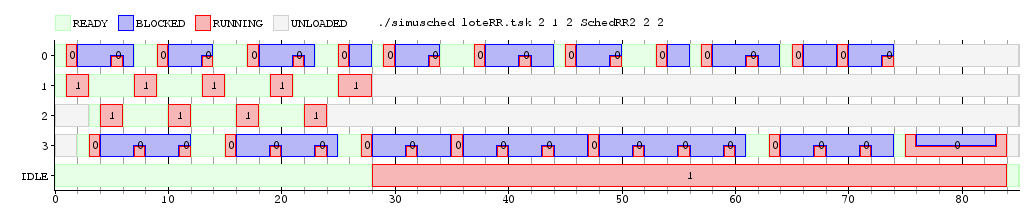
\includegraphics[width=\textwidth,height=3.0in,keepaspectratio
]{imagenes/ej8/2eje1.png} \\
\begin {flushleft}
\textbf{Figura 12:} Diagrama de Gantt para la ejecuci\'on del lote de tareas bajo 2 n\'ucleos con quantums de 2 y 2 ciclos respectivamente. En un Scheduler Round Robin sin migración de procesos.
\end{flushleft}	
 
  
  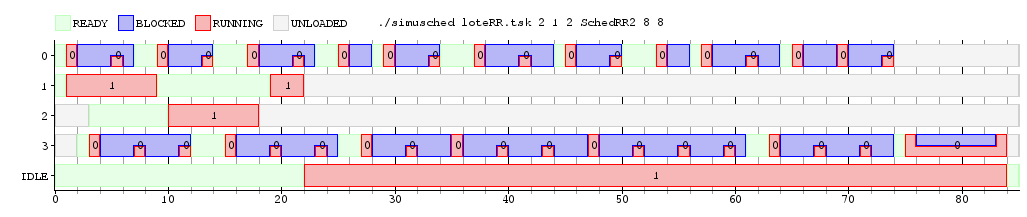
\includegraphics[width=\textwidth,height=3.0in,keepaspectratio
]{imagenes/ej8/2eje2.png} \\
\begin {flushleft}
\textbf{Figura 13:} Diagrama de Gantt para la ejecuci\'on del lote de tareas bajo 2 n\'ucleos con quantums de 8 y 8 ciclos respectivamente. En un Scheduler Round Robin sin migración de procesos.
\end{flushleft}	

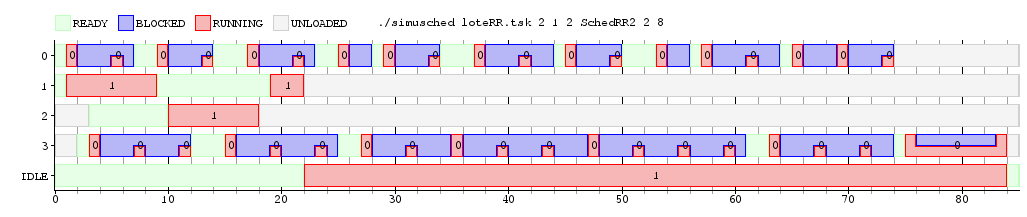
\includegraphics[width=\textwidth,height=3.0in,keepaspectratio
]{imagenes/ej8/2eje3.png} \\
\begin {flushleft}
\textbf{Figura 14:} Diagrama de Gantt para la ejecuci\'on del lote de tareas bajo 2 n\'ucleos con quantums de 2 y 8 ciclos respectivamente. En un Scheduler Round Robin sin migración de procesos.
\end{flushleft}	

\bigskip
Y para las tareas: 
  
 \begin{codesnippet}
	\begin{verbatim}
 TaskCPU 7
@2:
TaskCPU 6
@1:
TaskCPU 10
@3:
TaskCPU 4
	\end{verbatim}
	\end{codesnippet}
	
Obtuvimos los siguientes resultados:\\
	
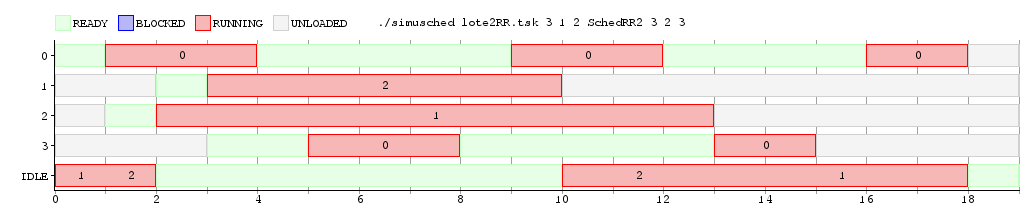
\includegraphics[width=\textwidth,height=3.0in,keepaspectratio
]{imagenes/ej8/2eje4.png} \\
\begin {flushleft}
\textbf{Figura 15:} Diagrama de Gantt para la ejecuci\'on del lote de tareas bajo 3 n\'ucleos con quantums de 3, 2 y 3 ciclos respectivamente. En un Scheduler Round Robin sin migración de procesos.
\end{flushleft}	
	

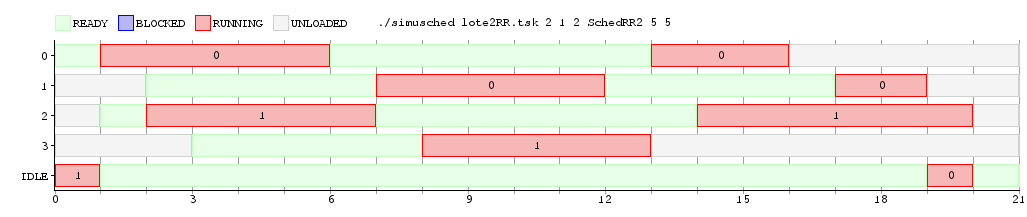
\includegraphics[width=\textwidth,height=3.0in,keepaspectratio
]{imagenes/ej8/2eje6.png} \\
\begin {flushleft}
\textbf{Figura 17:}Diagrama de Gantt para la ejecuci\'on del lote de tareas bajo 2 n\'ucleos con quantums de 5 y 5 ciclos respectivamente. En un Scheduler Round Robin sin migración de procesos.
\end{flushleft}	
 
\newpage
 \subsection{Ejercicio 9:  Ejecuci\'on lote de tareas}
\textit{Dise\~nar un lote de tareas cuyo scheduling no sea factible para el algoritmo de prioridades fijas pero s\'i para el algoritmo de prioridades din\'amicas.}



\end{document}

